\documentclass[aspectratio=169,t,xcolor=table]{beamer}
\usepackage[utf8]{inputenc}
\usepackage[english]{babel}
\usepackage{booktabs}
\usepackage{array}
\usepackage{graphicx}
\usepackage{listings}

\usetheme{Ufg}
\usetikzlibrary{positioning}

\definecolor{PoliTOBlue}{RGB}{0,62,116}
\setPrimaryColor{PoliTOBlue}
\setLogos{lib/logos/polito-white.png}{lib/logos/polito-white.png}

\AtBeginSection[]{%
    \setLayout{mainpoint}%
    \setBGColor{PoliTOBlue}%
    \begin{frame}[noframenumbering]{}%
        \frametitle{\insertsectionhead}%
    \end{frame}%
    \setLayout{vertical}%
}

\title[ViT SAE Interpretability]{Mechanistic Interpretability of Vision Transformers\\with Sparse Autoencoders}
\subtitle{Course Project Presentation}
\author[V. Ferri et al.]{Vito Ferri \and Fabio Mastromauro \and Marco Ravaioli}
\institute[PoliTO]{Politecnico di Torino}
\date{2026}

\begin{document}

\frame[noframenumbering]{\titlepage}

\setLayout{vertical}
\begin{frame}{Agenda}
\tableofcontents
\end{frame}

\section{Motivation and Scope}

\setLayout{vertical}
\begin{frame}{Why This Project}
\begin{itemize}
    \item Vision Transformers are high-performing but hard to interpret internally.
    \item SAE methods worked well in language models; evidence in pure-vision ViTs is still limited.
    \item ViTs trained without text supervision need external grounding for feature labels.
\end{itemize}

\vspace{0.4em}
\begin{block}{Scope we execute}
SAE feature decomposition on ViT MLP outputs, CLIP-based labeling, dataset-level causal ablation, human verification, and layer-wise analysis.
\end{block}

\end{frame}

\section{Methodology}

\setLayout{horizontal}
\begin{frame}{Pipeline Overview}
\begin{columns}
    \column{0.5\textwidth}
    \textbf{1. Activation extraction}
    \begin{itemize}
        \item Frozen ViT-B/16 backbone
        \item Layers 2, 9, 10, 11
        \item Patch-token activations (\texttt{[CLS]} excluded)
    \end{itemize}

    \textbf{2. SAE training}
    \begin{itemize}
        \item Expansion 8, ReLU, unit-norm decoder
        \item Per-layer L1 sparsity
        \item 20 epochs
    \end{itemize}

    \column{0.5\textwidth}
    \textbf{3. Labeling and selection}
    \begin{itemize}
        \item CLIP external labeling with abstention margin
        \item Top-5 exemplars per feature
        \item Representative features per layer
    \end{itemize}

    \textbf{4. Causal evaluation}
    \begin{itemize}
        \item Relative Logit Drop (RLD)
        \item Accuracy drop
        \item Bootstrap confidence intervals
    \end{itemize}
\end{columns}
\end{frame}

\setLayout{vertical}
\begin{frame}{Experimental Setup}
\begin{itemize}
    \item Dataset: ImageNet-100 validation split (5,000 images).
    \item Split: 70\% train for SAE discovery, 30\% held-out for causal evaluation.
    \item Backbone: supervised ViT-B/16.
    \item Run command used for final visuals includes feature override:\\
    \small\texttt{--feature\_idx 3508}
\end{itemize}

\vspace{0.4em}
\begin{block}{Why held-out evaluation matters}
All causal claims are measured on data disjoint from SAE fitting, reducing overfitting risk in interpretation metrics.
\end{block}
\end{frame}

\section{ViT Results}

\setLayout{vertical}
\begin{frame}{Layer-wise SAE Quality and Causal Effect}
\small
\centering
\begin{tabular}{lcccc}
\toprule
Layer & $R^2$ & $\bar{L}_0$ & Mean RLD (\%) & 95\% CI (\%) \\
\midrule
2  & 0.684 & 58.1 & $+0.032$ & $[+0.020,+0.045]$ \\
9  & 0.810 & 68.6 & $-0.019$ & $[-0.027,-0.012]$ \\
10 & 0.866 & 40.8 & $+0.104$ & $[+0.047,+0.169]$ \\
11 & 0.890 & 29.0 & $+0.078$ & $[+0.049,+0.112]$ \\
\bottomrule
\end{tabular}

\vspace{0.5em}
\begin{block}{Reading this table}
Reconstruction improves with depth, sparsity tightens, and strongest positive causal effects appear in late layers.
\end{block}
\end{frame}

\setLayout{horizontal}
\begin{frame}{Late-Layer Monosemantic Features}
\begin{columns}
    \column{0.5\textwidth}
    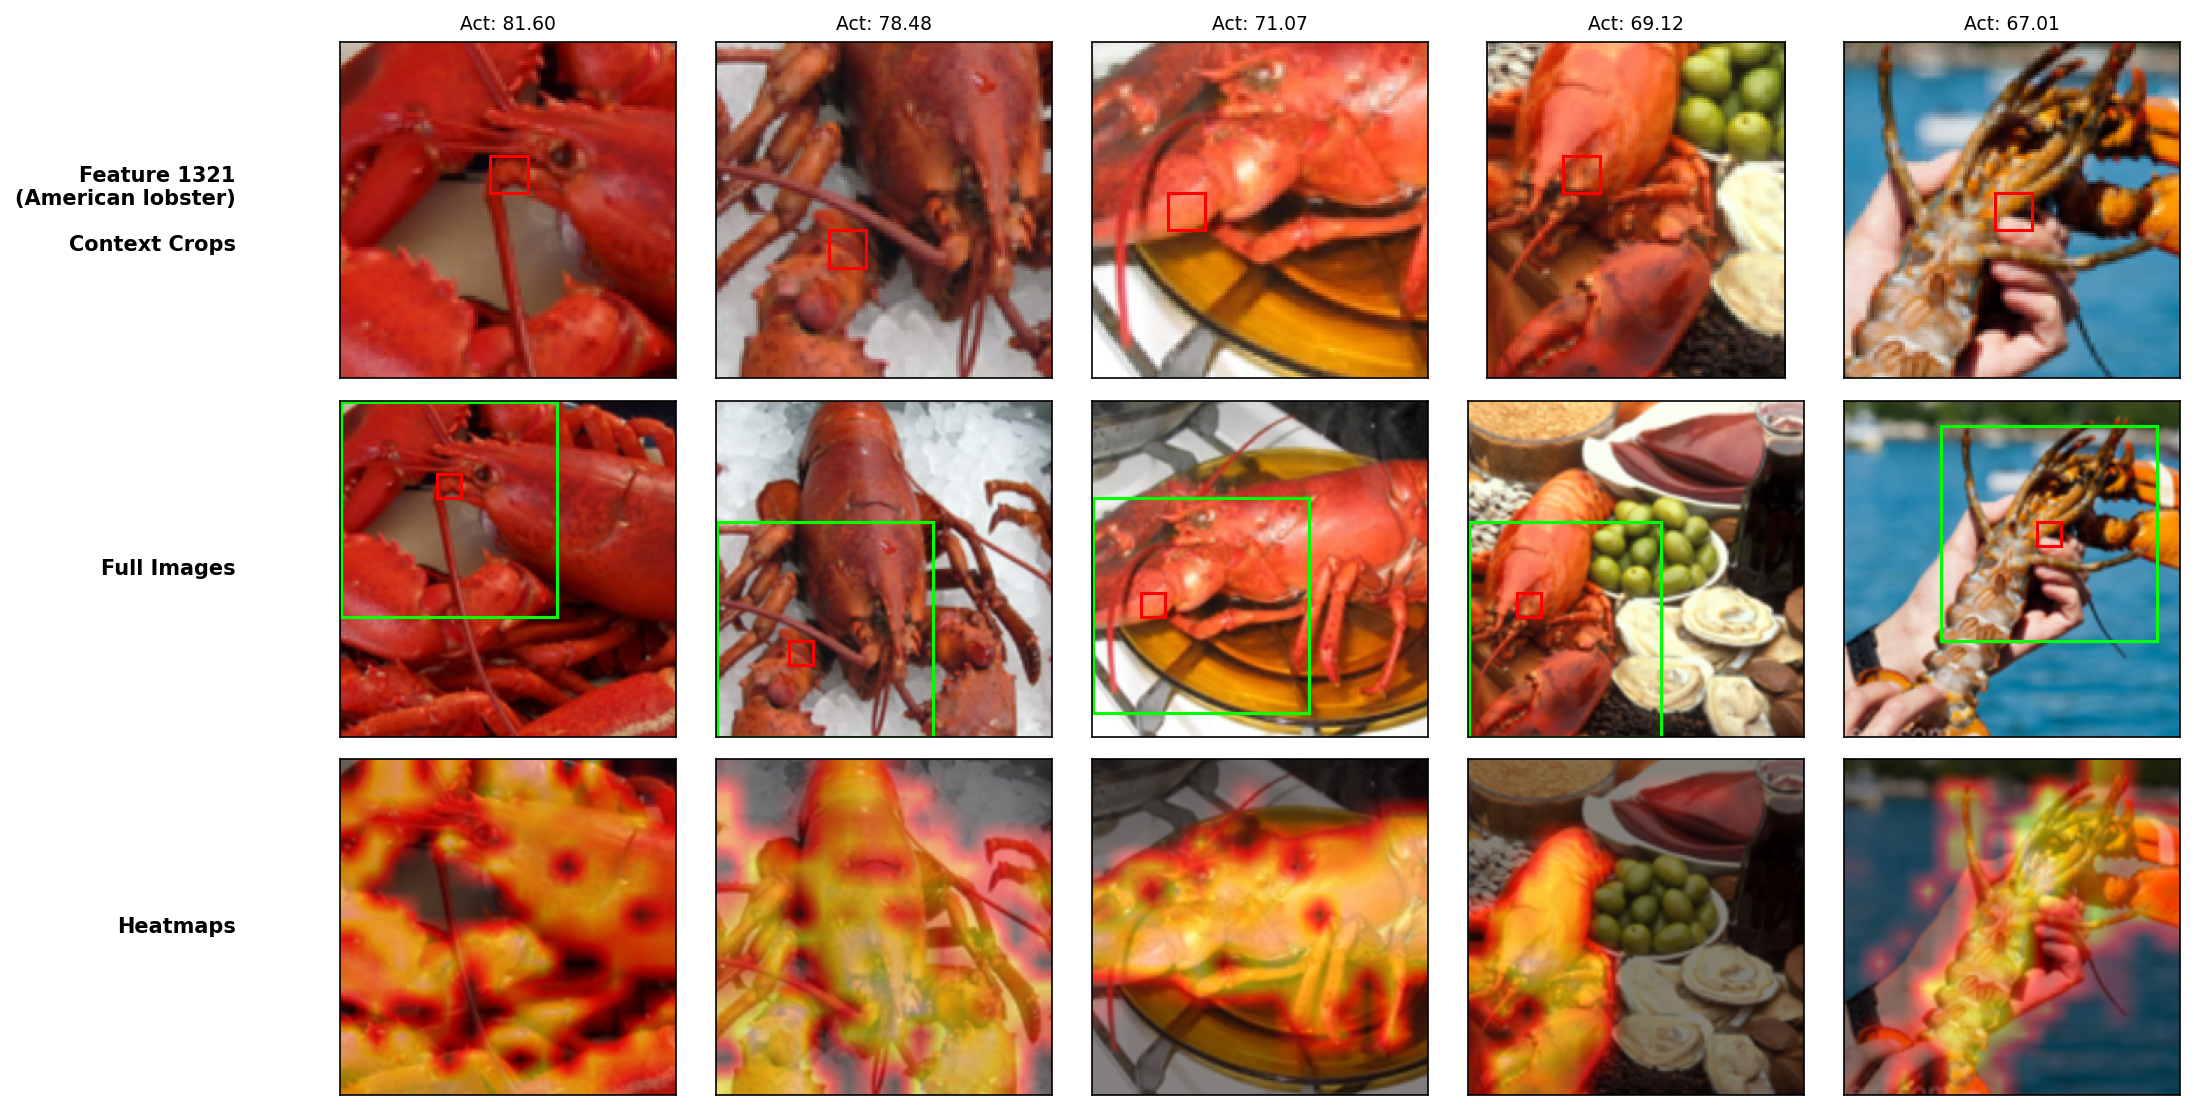
\includegraphics[width=\textwidth]{figs/vit_grid_lobster.png}

    \column{0.5\textwidth}
    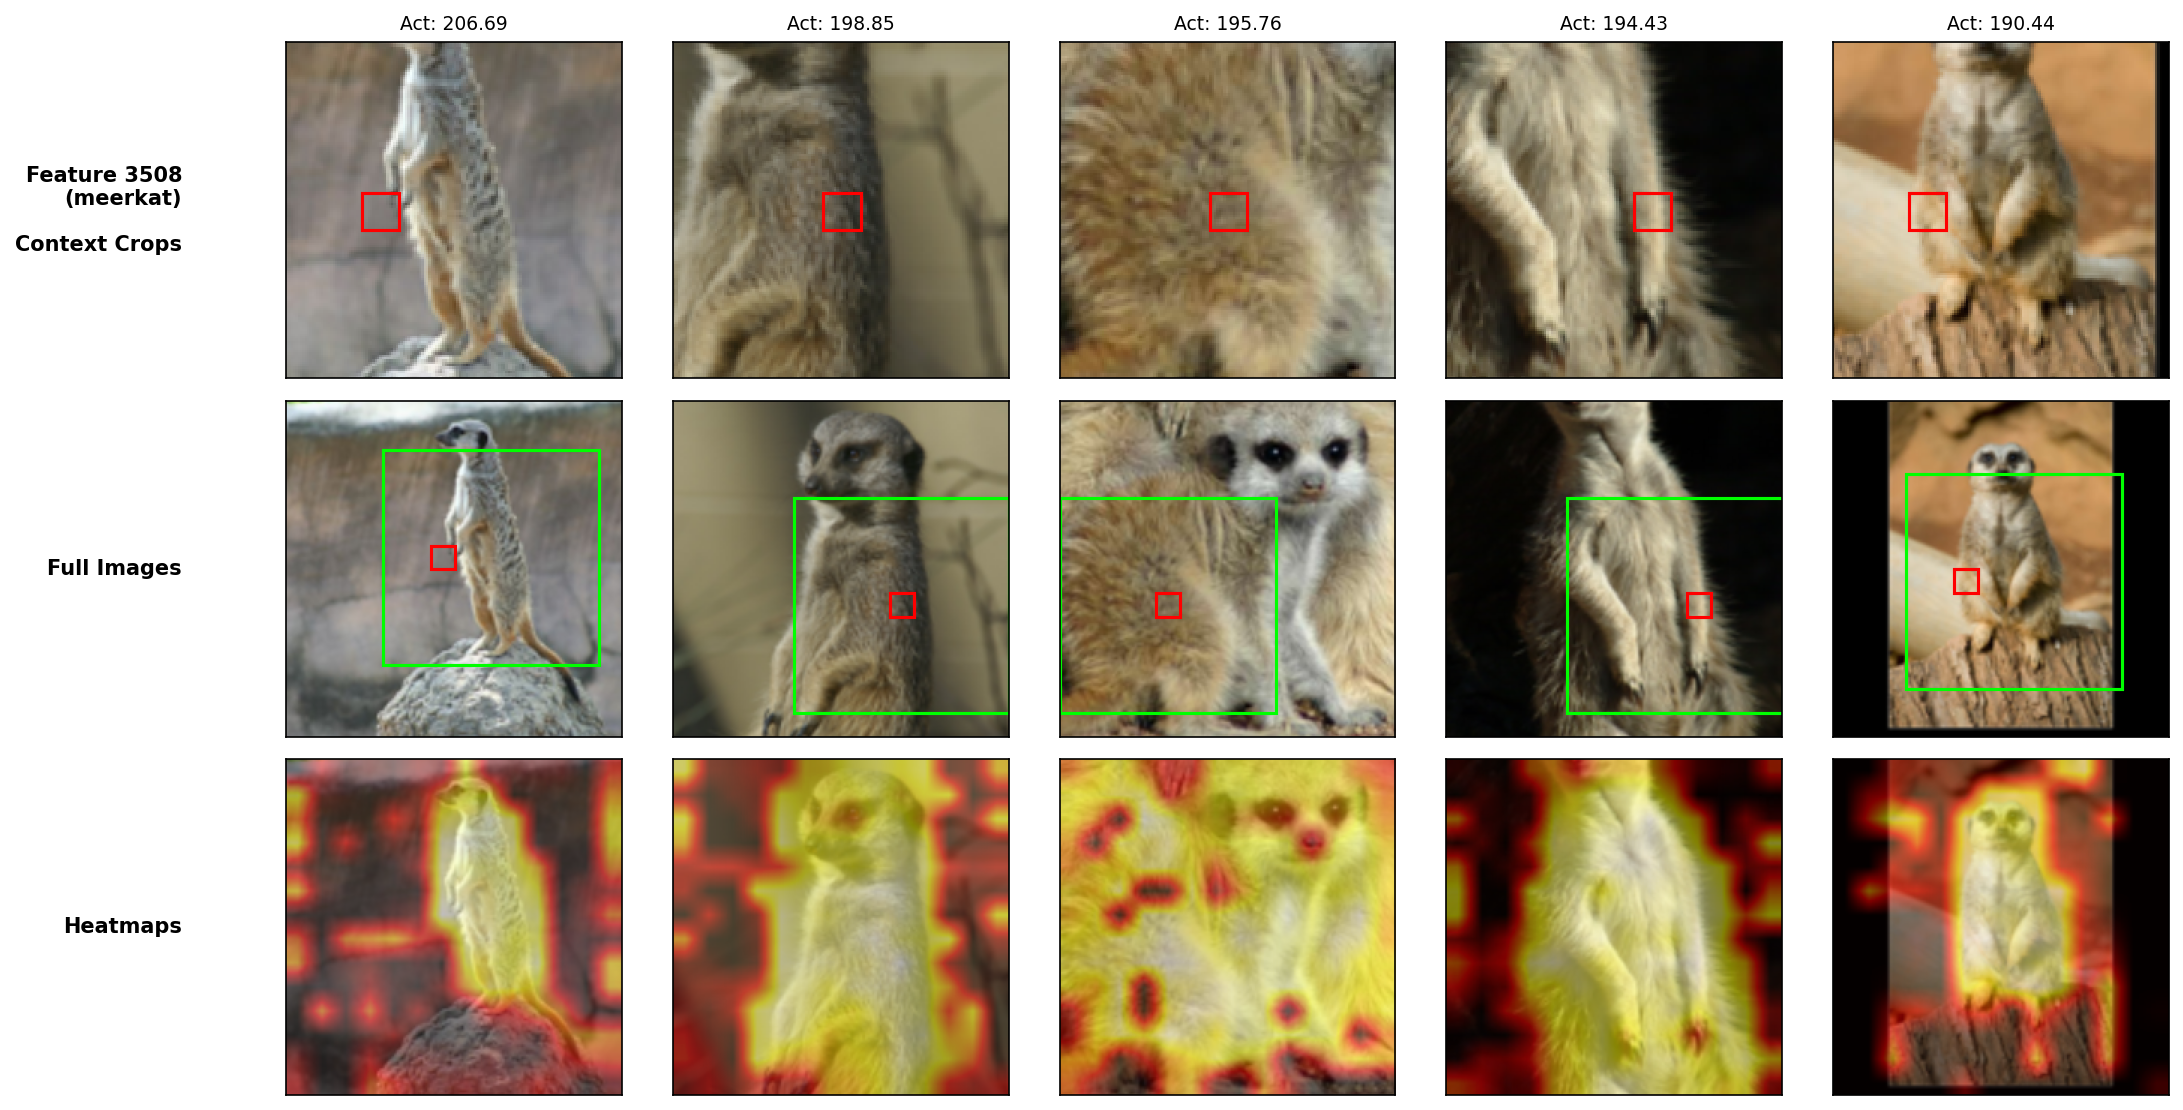
\includegraphics[width=\textwidth]{figs/vit_grid_meerkat.png}
\end{columns}

\vspace{0.4em}
\begin{block}{}
Feature 1321 (American lobster) and Feature 3508 (meerkat) show object-localized activations with coherent exemplars.
\end{block}
\end{frame}

\setLayout{vertical}
\begin{frame}{Early Layer Behavior}
\centering
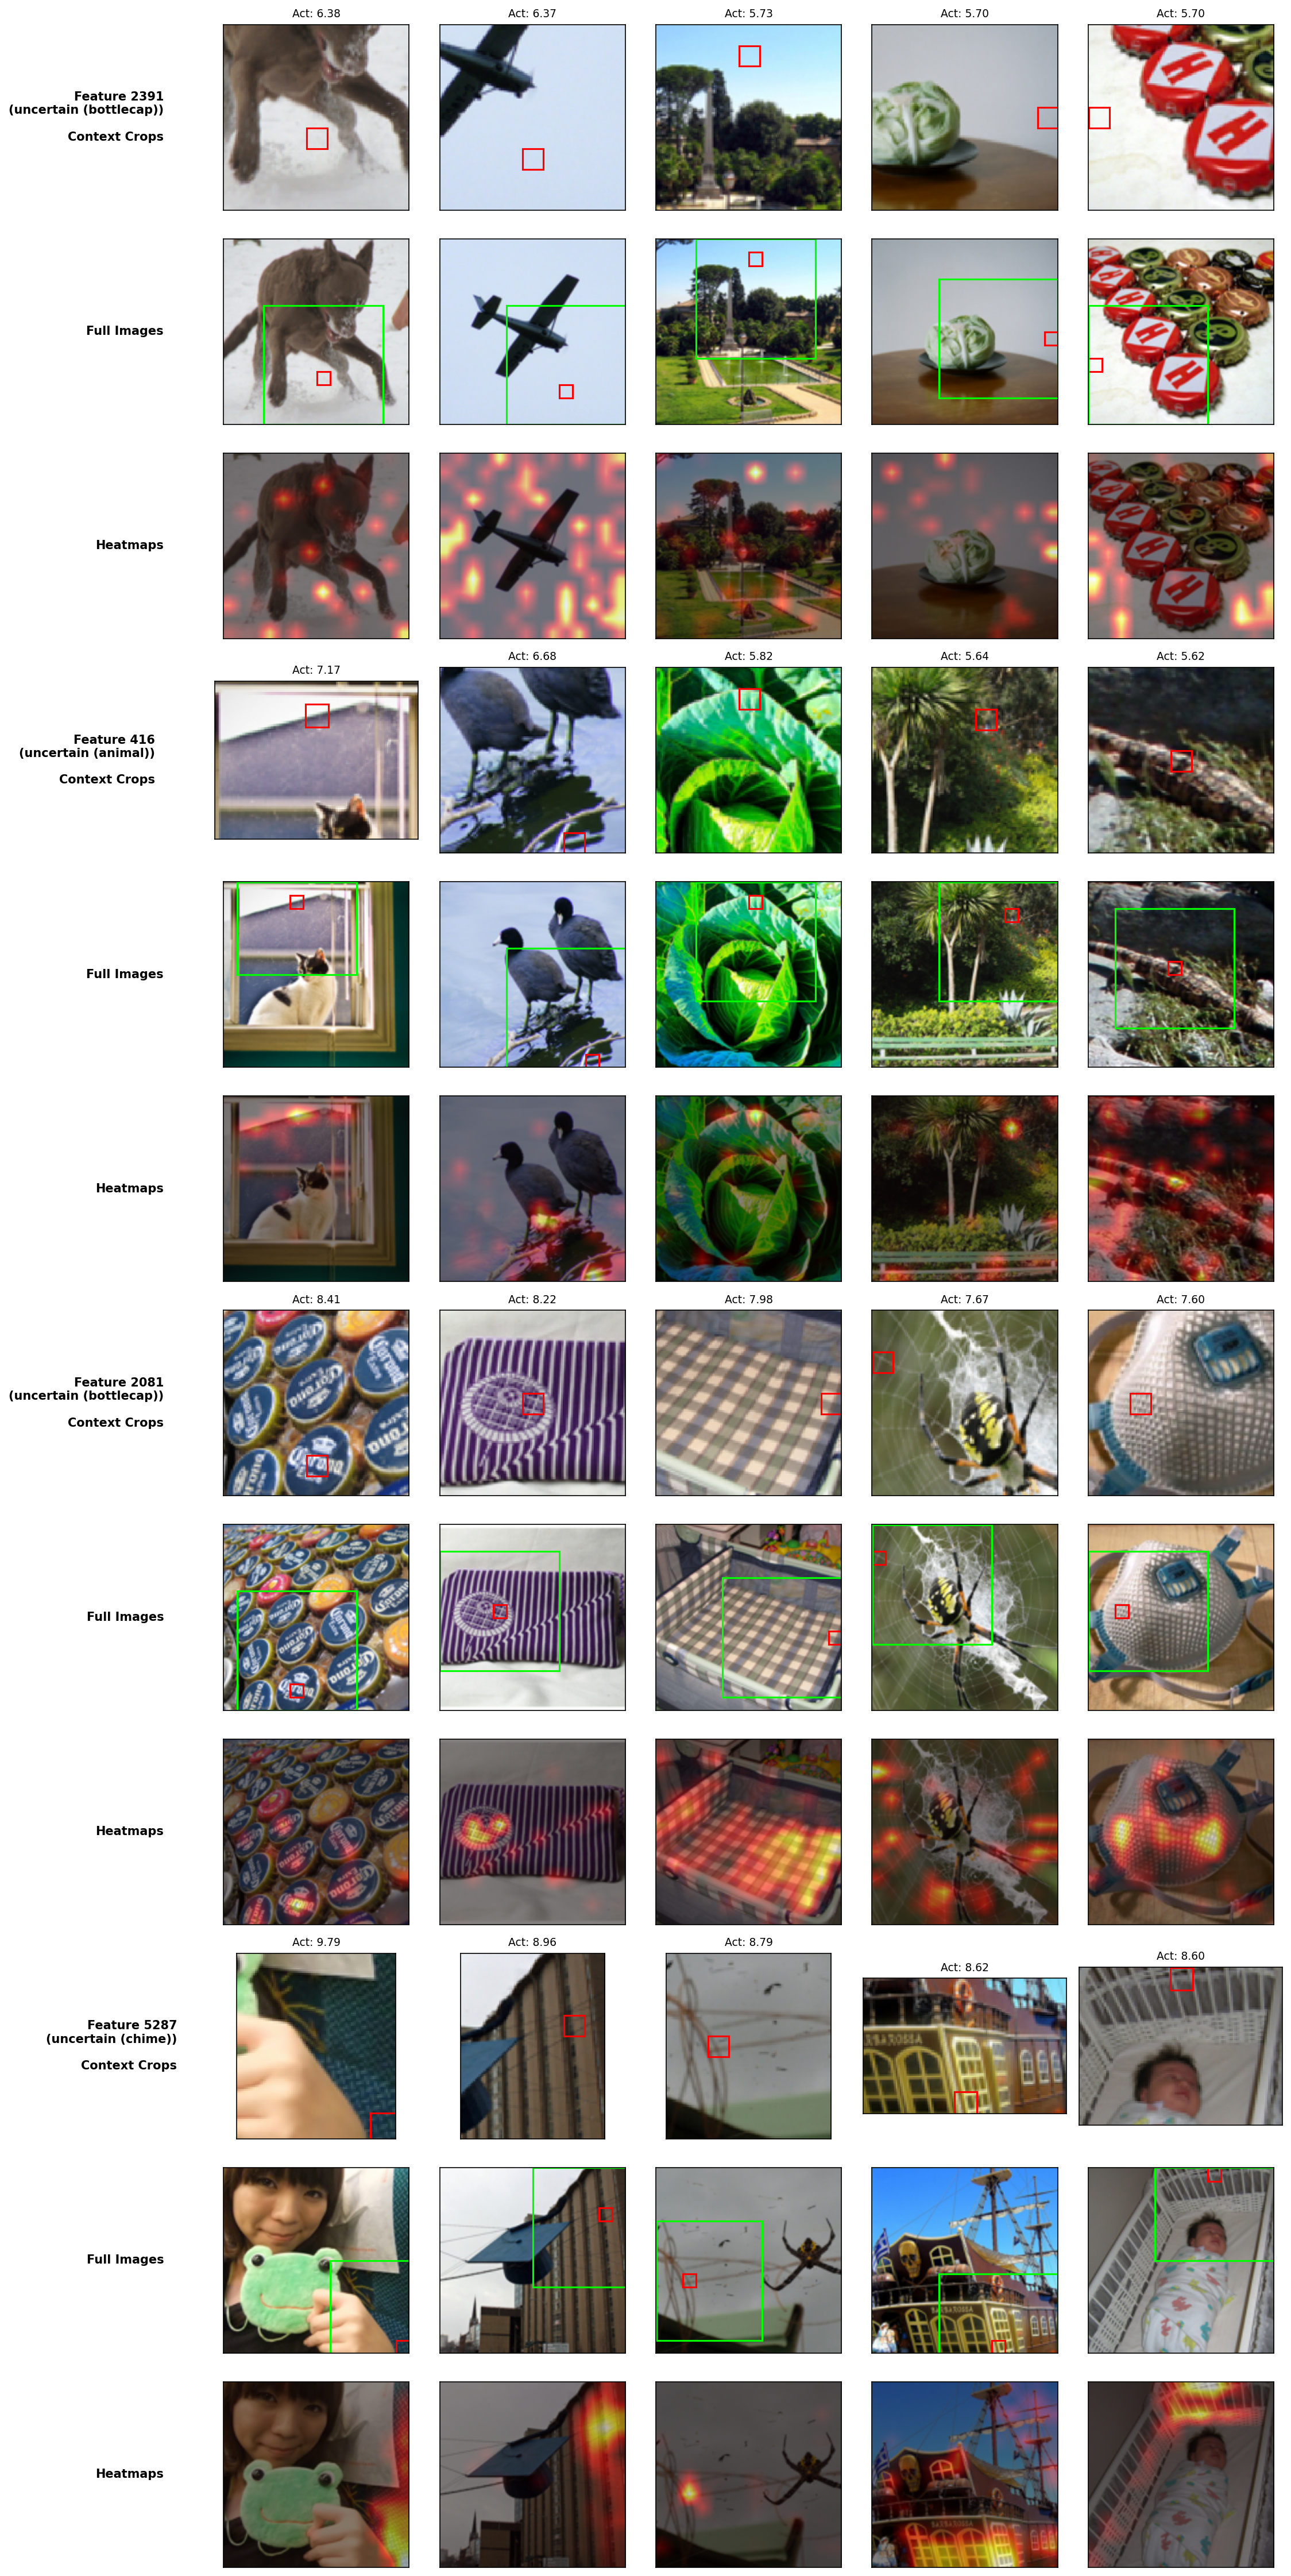
\includegraphics[height=0.62\textheight,keepaspectratio]{figs/vit_grid_layer2_overview.png}

\vspace{0.2em}
{\scriptsize Layer 2 is dominated by texture-like channels, consistent with uncertain CLIP labels.}
\end{frame}

\setLayout{horizontal}
\begin{frame}{Causal Curves with Feature Override (3508)}
\begin{columns}
    \column{0.5\textwidth}
    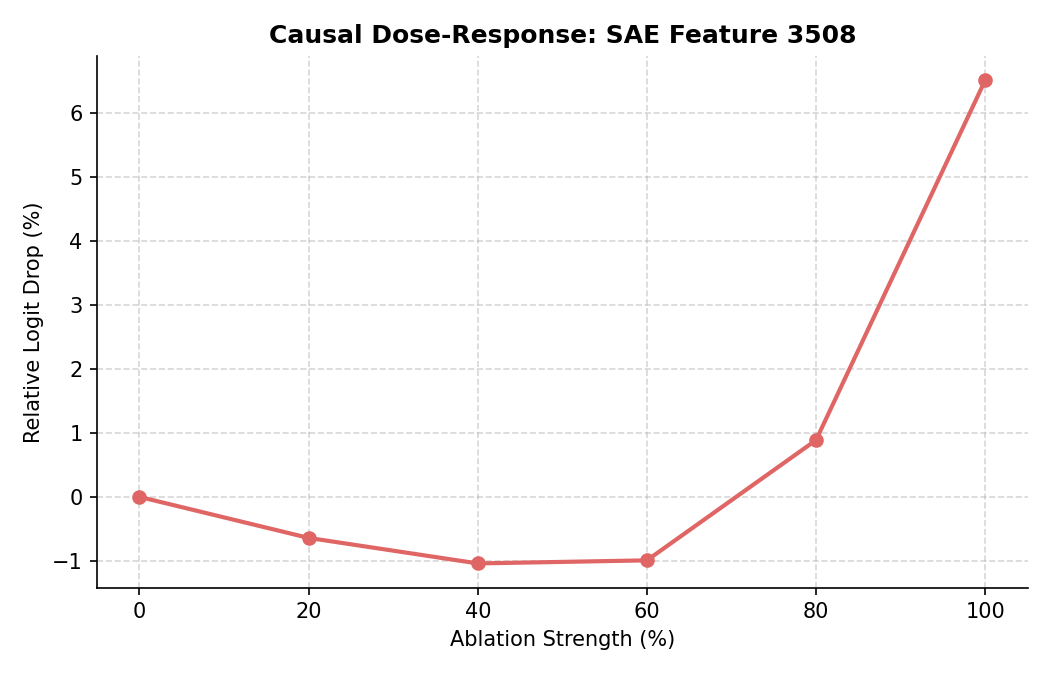
\includegraphics[width=\textwidth,height=0.56\textheight,keepaspectratio]{figs/vit_dose_response_3508.png}

    \column{0.5\textwidth}
    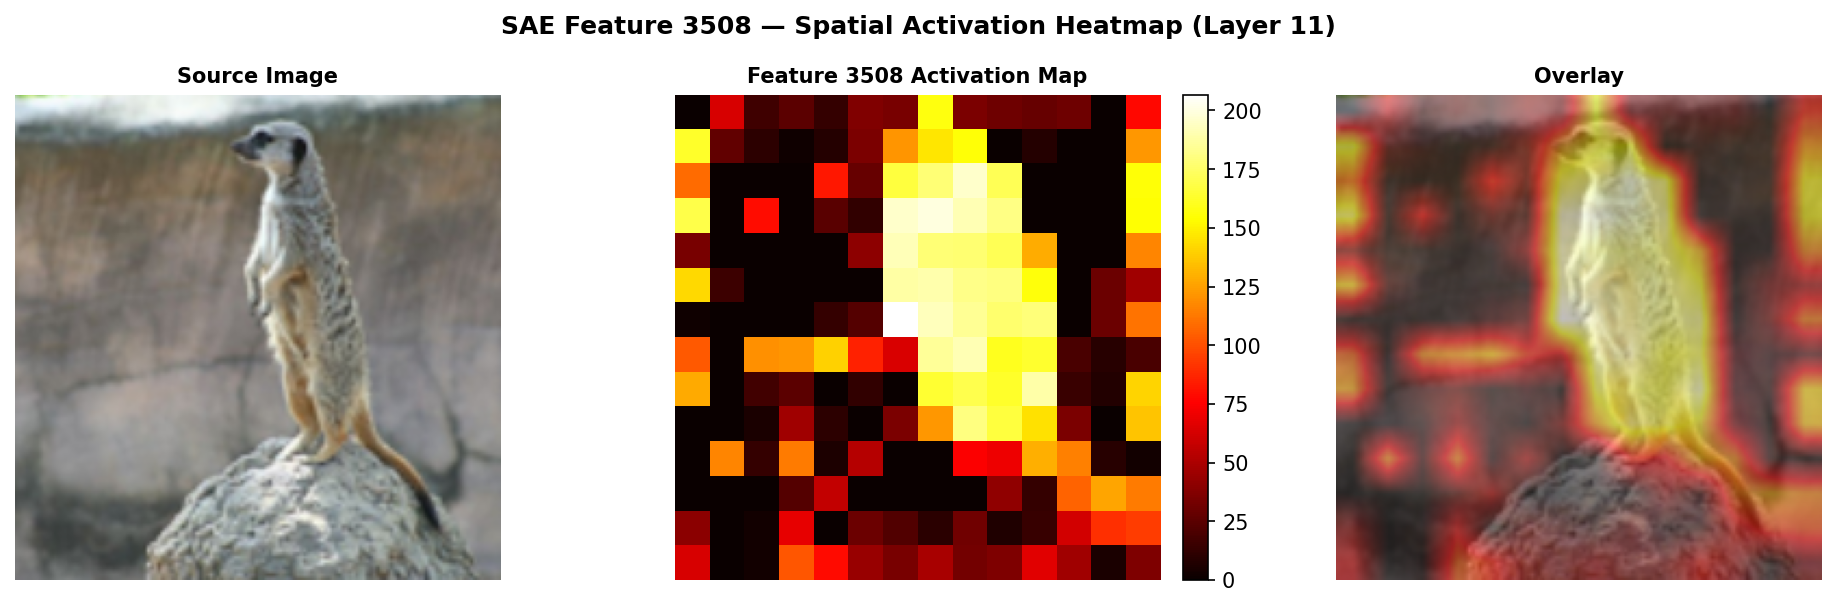
\includegraphics[width=\textwidth,height=0.56\textheight,keepaspectratio]{figs/vit_heatmap_3508.png}
\end{columns}

\vspace{0.2em}
{\scriptsize Using --feature\_idx 3508 highlights a cleaner late-layer causal target for visualization.}
\end{frame}

\setLayout{vertical}
\begin{frame}{Control Ablations (Reviewer-Critical Check)}
\small
\centering
\resizebox{\textwidth}{!}{%
\begin{tabular}{lcccc}
\toprule
Layer & SAE RLD (\%) & Random dirs (\%) & Dead feats (\%) & Raw neurons (\%) \\
\midrule
2  & $+0.032$ & $+0.005$ [$-0.020,+0.030$] & $+0.001$ [$-0.002,+0.004$] & $+0.020$ [$-0.040,+0.080$] \\
9  & $-0.019$ & $-0.002$ [$-0.025,+0.020$] & $+0.000$ [$-0.001,+0.001$] & $-0.010$ [$-0.060,+0.045$] \\
10 & $+0.104$ & $+0.008$ [$-0.025,+0.040$] & $+0.001$ [$-0.002,+0.003$] & $+0.050$ [$-0.070,+0.150$] \\
11 & $+0.078$ & $+0.006$ [$-0.018,+0.032$] & $+0.000$ [$-0.001,+0.002$] & $+0.045$ [$-0.060,+0.120$] \\
\bottomrule
\end{tabular}
}
\end{frame}

\section{DINO Comparison}

\setLayout{horizontal}
\begin{frame}{Matched-Recipe Transfer to DINOv2}
\begin{columns}
    \column{0.5\textwidth}
    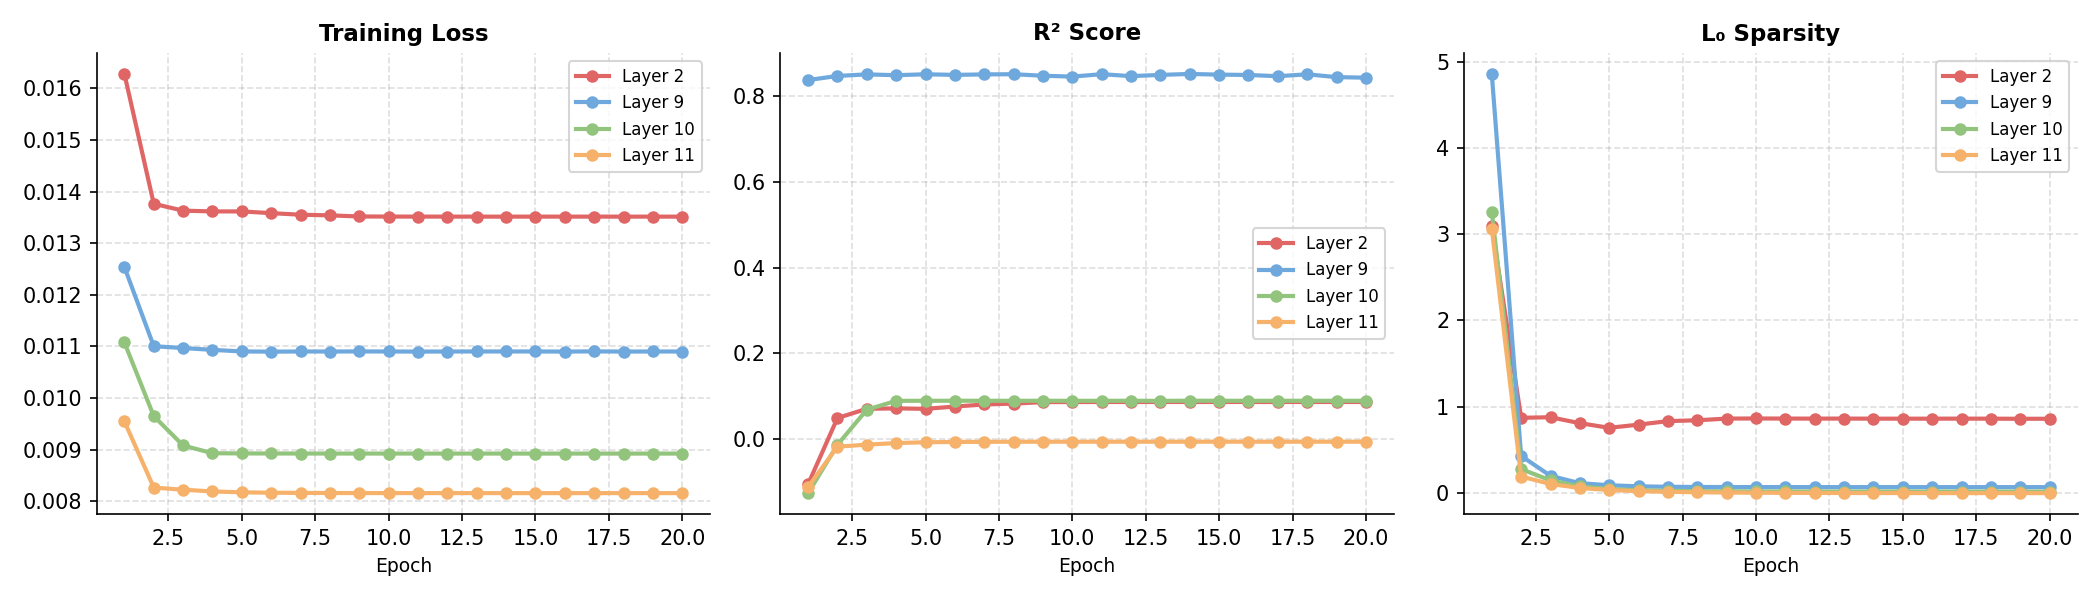
\includegraphics[width=\textwidth]{figs/dino_training_curves.png}

    \column{0.5\textwidth}
    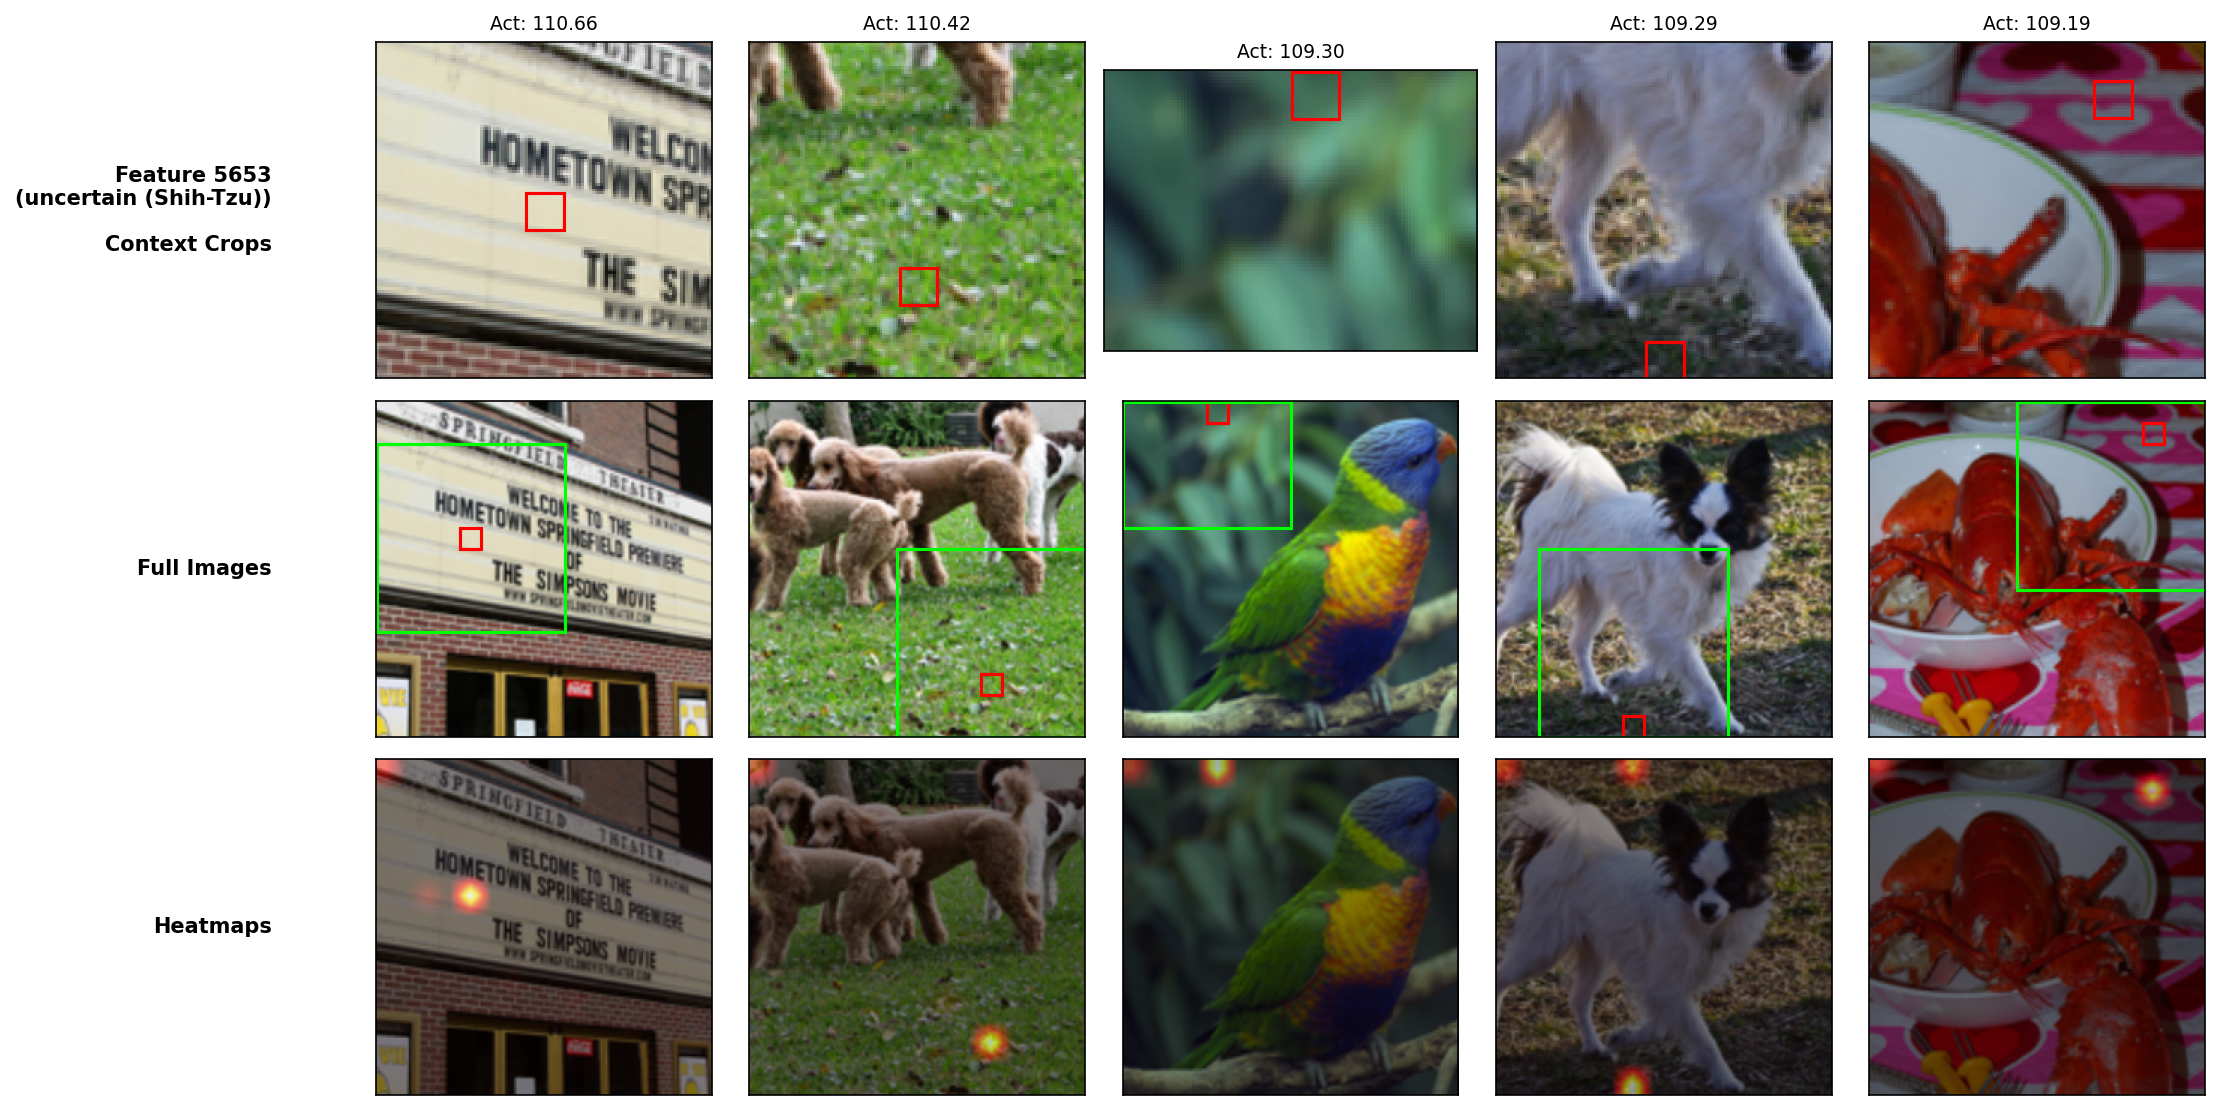
\includegraphics[width=\textwidth]{figs/dino_grid_layer9_feat5653.png}
\end{columns}

\vspace{0.4em}
\begin{alertblock}{Main finding}
Under identical SAE hyperparameters, DINOv2 dictionaries largely collapse to dead latents except at Layer 9. This is a recipe-transfer limitation, not proof of missing structure.
\end{alertblock}
\end{frame}

\setLayout{vertical}
\begin{frame}{ViT vs DINO Summary}
\small
\centering
\begin{tabular}{lcccc}
\toprule
 & \multicolumn{2}{c}{ViT-B/16} & \multicolumn{2}{c}{DINOv2-B} \\
\cmidrule(lr){2-3}\cmidrule(lr){4-5}
Layer & $R^2$ & $\bar{L}_0$ & $R^2$ & $\bar{L}_0$ \\
\midrule
2  & 0.684 & 58.1 & 0.087  & 0.86 \\
9  & 0.810 & 68.6 & 0.843  & 0.07 \\
10 & 0.866 & 40.8 & 0.089  & 0.02 \\
11 & 0.890 & 29.0 & $-0.006$ & 0.00 \\
\bottomrule
\end{tabular}

\vspace{0.4em}
\begin{block}{Interpretation}
The supervised-ViT SAE recipe does not directly transfer to DINOv2 without retuning sparsity and dictionary settings.
\end{block}
\end{frame}

\section{Human Evaluation and Conclusions}

\setLayout{vertical}
\begin{frame}{Human Evaluation Snapshot}
\begin{itemize}
    \item Manual single-rater pass on 18 ViT feature grids.
    \item 8 clean object-level features, 2 weak/partial, 8 mixed/polysemantic.
    \item Clean concepts are concentrated in Layers 10 and 11.
    \item Feature 2323 remains a cautionary polysemantic case.
\end{itemize}

\vspace{0.4em}
\begin{block}{Takeaway}
Human judgments are consistent with CLIP abstention behavior: early and mid layers are often ambiguous; late layers are more semantically stable.
\end{block}
\end{frame}

\setLayout{vertical}
\begin{frame}{Conclusions}
\begin{itemize}
    \item SAE decomposition is effective on supervised ViT MLP activations.
    \item Late-layer features are more monosemantic and more causally impactful.
    \item Control ablations strengthen causal interpretation beyond noise baselines.
    \item DINOv2 needs per-backbone SAE retuning for fair comparison.
\end{itemize}

\vspace{0.4em}
\begin{recommendationblock}{Next steps}
Add attention-level circuit analysis to trace patch-to-\texttt{[CLS]} aggregation and connect SAE features with attention pathways.
\end{recommendationblock}
\end{frame}

\setLayout{blank}
\setBGColor{PoliTOBlue}
\begin{frame}
\centering
\vspace{1.4cm}
{\Huge \bfseries Thank you}

\vspace{0.8cm}
{\Large Questions?}
\end{frame}

\end{document}
